%&tex
\documentclass{article}

\usepackage{graphicx}[draft]
\usepackage{color}
\graphicspath{{./img/}}
\usepackage{geometry}
\usepackage{hyperref}
\usepackage{subcaption}
\usepackage{float}

\floatplacement{figure}{htb}

\title{Exercise 04 -- Normalization}
\author{Stewart Johnston\\
  {CIS 215 -- Database Design}\\
  {NCMC}\\
  {\texttt{johnstons1@student.ncmich.edu}}
}
\date{\today}

\begin{document}

\maketitle

The invoice given us to normalize the data and put into a relational
database is not naturally in a normalized form. Several different tables
need to be split off in order to accurately model the data while also
making it simple to work on.

\begin{figure}
	\centering
	\includegraphics[width=\textwidth]{norm5.jpg}
	\caption{Order Form serving as source document for analysis}
\end{figure}

\section{First Normal Form}

The tenets of first normal form include:
\begin{enumerate}
	\item Atomic values for any given field of any given tuple. In
		more plain English, for any intersection of row and
		column, therein will be only one value of the
		attribute's type or domain.
		
		It is often phrased as having ``No Repeating Groups''.
		The important part of this is consideration is that if
		multiple pieces of data are introduced with the same
		type/domain, they must be uniquely identifiable in
		the row without asking for the nth instance of that
		attribute.  ``Address\_1'' and ``Address\_2'', for
		example, would not be appropriate.  However,
		``shipping\_address'' and ``billing\_address'' may be
		appropriate, depending on the business rules and the
		cardinality of the relationship.
		
		A 1:n cardinality, for instance, would not be
		appropriate to denormalize in this way. If any one
		entity had an exact number of named variants of the same
		domain (e.g. work and cell number), pulling them into
		the main relation may be appropriate. Your mileage may
		vary.

	\item Each tuple in the relation must be uniquely identifiable
		with a primary key. A primary key can be an arbitrary
		auto-incrementing value, which is quite often the case.
		A primary key can be composed of multiple pieces of a
		tuple's data, as long as this data will never collide on
		multiple tuples. It is recommended that this primary key
		be composed of values which are likely never to change
		but also do not have confidentiality/security
		requirements. (e.g., a birth date in combination with
		other data may be appropriate, but a social security
		number would not be).

	\item Groups of similar data should be wrapped in their own
		tables, \emph{especially} if they have any cardinality
		other than 1:1 with any other data belonging to the same
		entity.

		In the exercise, individual products have a many:many
		cardinality with order forms, so products are best
		stored in their own table. The quantity of any given
		product on any given order form is best stored as an
		attribute of an associative table between the order form
		primary key and the product primary key, since those are
		the determinants of the quantity.

\end{enumerate}

To meet this criteria for first normal form, I examined only the
cardinality between pieces of data and how they related as entities to
the order form as an entity.

\section{Second Normal Form}

Second Normal Form requires firstly that data be in First Normal Form,
and additionally that non-key data be completely functionally dependent
on the primary key. A Functional Dependency occurs between two
attributes when for any given value of the determinant, the dependent
will only have one possible value at any given time. So to say,
Functional Dependency is like a one-way 1:1 cardinality between
individual attributes of a relation. The reverse need not be true; a
duplicate value of dependent can occur in many places, being referenced
by different determinants, but for any value of determinant, only one
value of dependant exists.

A Transitive Dependency is like the transitive property in logic or
algebra. E.g, if A implies B, which implies C, then by the transitive
property means A implies C.

Transitive Functional Dependencies are legal in 2NF, so no structural
changes need to be made to the tables. However, it is useful to
recognize where transitive functional dependencies are, which can be
seen in the Second Normal Form subgraph. Any node which has arrows into
and out of it is a point of transitive dependency.

\begin{figure}
	\centering
	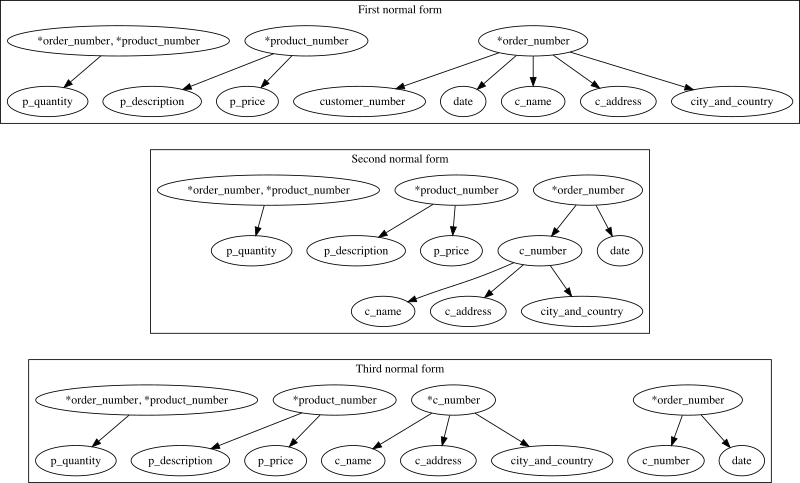
\includegraphics[width=\textwidth]{Ex04-Normalization-Stewart_Johnston.png}
	\caption{Dependency graph for First, Second, and Third normal
	forms}
\end{figure}

\section{Third Normal Form}

Third Normal Form, like the normal forms before it, requires that data
satisfy the prior Normal Form, and that no attributes which are not part
of the primary key have a Transitive Dependency on the primary key. To
that end, the changes made to the structure of the data to make it
comply with 3NF are to move any transitive dependencies into their own
relations. In the Exercise, this can be done by splitting off the
customer number and its dependents -- name, address, and city/country --
into their own relation. Then the customer number becomes the primary
key for its own relation, and it is referenced as a foreign key by the
order form relation.

\end{document}
